\documentclass{article}
\usepackage{tikz}
\usetikzlibrary{shapes.geometric}

\begin{document}

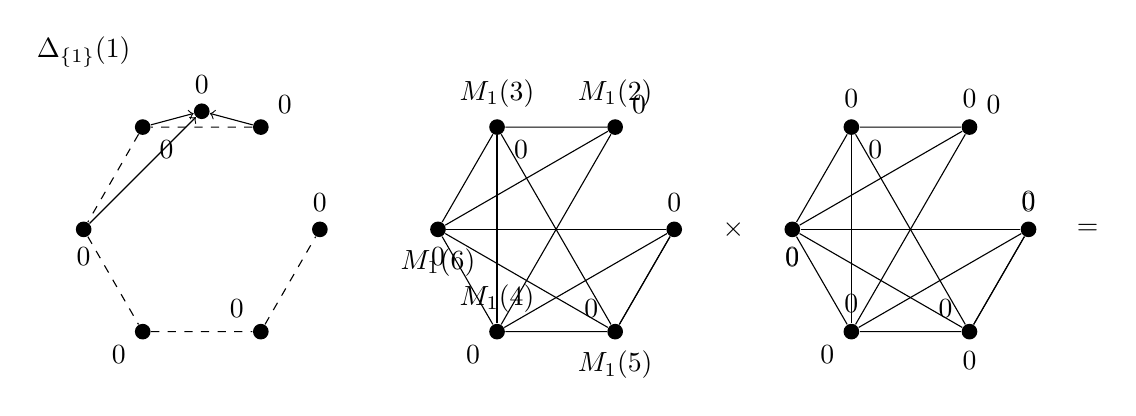
\begin{tikzpicture}[scale=1.5]
    % Define the vertices of the hexagon
    \foreach \i in {1,...,6} {
        \node[circle,fill,inner sep=2pt,label={90-60*\i}:0] (v\i) at ({60*\i}:1) {};
    }
    
    % Draw the hexagon
    \draw[dashed] (v1) -- (v2) -- (v3) -- (v4) -- (v5) -- (v6) -- cycle;
    
    % Draw the triangle
    \node[circle,fill,inner sep=2pt,label={90}:0] (t1) at (0,1) {};
    \draw[->] (v1) -- (t1);
    \draw[->] (v2) -- (t1);
    \draw[->] (v3) -- (t1);
    
    % Label the triangle
    \node at (-1,1.5) {$\Delta_{\{1\}}(1)$};
    
    % Second diagram
    \begin{scope}[xshift=3cm]
        % Define the vertices of the hexagon
        \foreach \i in {1,...,6} {
            \node[circle,fill,inner sep=2pt,label={90-60*\i}:0] (m\i) at ({60*\i}:1) {};
        }
        
        % Draw the hexagon
        \draw (m1) -- (m2) -- (m3) -- (m4) -- (m5) -- (m6) -- cycle;
        
        % Draw the lines connecting the vertices
        \draw (m1) -- (m3);
        \draw (m1) -- (m4);
        \draw (m2) -- (m4);
        \draw (m2) -- (m5);
        \draw (m3) -- (m5);
        \draw (m3) -- (m6);
        \draw (m4) -- (m6);
        \draw (m5) -- (m6);
        
        % Label the vertices
        \node at (m1) [label=above:$M_1(2)$] {};
        \node at (m2) [label=above:$M_1(3)$] {};
        \node at (m3) [label=below:$M_1(6)$] {};
        \node at (m4) [label=above:$M_1(4)$] {};
        \node at (m5) [label=below:$M_1(5)$] {};
        
        % Third diagram
        \begin{scope}[xshift=3cm]
            % Define the vertices of the hexagon
            \foreach \i in {1,...,6} {
                \node[circle,fill,inner sep=2pt,label={90-60*\i}:0] (result\i) at ({60*\i}:1) {};
            }
            
            % Draw the hexagon
            \draw (result1) -- (result2) -- (result3) -- (result4) -- (result5) -- (result6) -- cycle;
            
            % Draw the lines connecting the vertices
            \draw (result1) -- (result3);
            \draw (result1) -- (result4);
            \draw (result2) -- (result4);
            \draw (result2) -- (result5);
            \draw (result3) -- (result5);
            \draw (result3) -- (result6);
            \draw (result4) -- (result6);
            \draw (result5) -- (result6);
            
            % Label the vertices
            \node at (result1) [label=above:$0$] {};
            \node at (result2) [label=above:$0$] {};
            \node at (result3) [label=below:$0$] {};
            \node at (result4) [label=above:$0$] {};
            \node at (result5) [label=below:$0$] {};
            \node at (result6) [label=above:$0$] {};
        \end{scope}
        
        % Label the multiplication
        \node at (1.5,0) {$\times$};
        \node at (4.5,0) {$=$};
    \end{scope}
\end{tikzpicture}

\end{document}